The expanded benchmark uses the same Apple M3 CPU, one numerical
thread and batch size one for seven model variants, after project training and
evaluation have stopped. One deterministic recording from each class and official
fold gives 250 unique five-second clips; three repetitions give 750 timed queries
per model in each pass. After observing different frontend times for CNNs with
identical processing, a post-hoc second pass reverses the model order. Both passes
are retained, giving 10,500 timed queries in total. Model, audio, software and
benchmark-source hashes match across passes, and all timed predictions match the
formal clean evaluations. Ten warm-ups precede each fold's panel. Total latency directly times
preprocessing, representation extraction, all-class scoring and argmax. Disk I/O,
model loading and one-off text preparation are excluded. Model-specific pinned
software environments are recorded. CNN latency uses seed 5305; its three-seed
accuracy analysis is separate. This is a two-order descriptive sensitivity on
one machine, not a randomised hardware study. The timing shift cannot be assigned
to a measured thermal or scheduling cause. In particular, differences among
identically shaped CNNs are not evidence that augmentation changes operation count.
\begin{table}[htbp]\centering\small
\caption{Balanced CPU panel: both timing passes. Medians and p95 values are in milliseconds. Serialized size is one fold's model (median across folds), or the CLAP checkpoint; it is not resident memory.}
\begin{tabular}{lrrrrr}\toprule Model / training & Median 1 & Median 2 & p95 1 & p95 2 & File (MB)\\\midrule
SVM / clean & 15.00 & 11.29 & 22.01 & 11.79 & 2.41 \\
SVM / WGN & 14.95 & 11.47 & 26.39 & 12.11 & 4.83 \\
SVM / semantic & 13.92 & 11.42 & 15.69 & 12.19 & 4.68 \\
CNN / clean & 3.07 & 2.44 & 3.61 & 2.59 & 0.16 \\
CNN / WGN & 4.83 & 2.43 & 6.42 & 2.64 & 0.16 \\
CNN / semantic & 2.97 & 2.48 & 3.17 & 2.68 & 0.16 \\
CLAP / single prompt & 69.30 & 50.86 & 97.44 & 53.04 & 1863.59 \\
\bottomrule\end{tabular}\end{table}

\begin{figure}[htbp]\centering
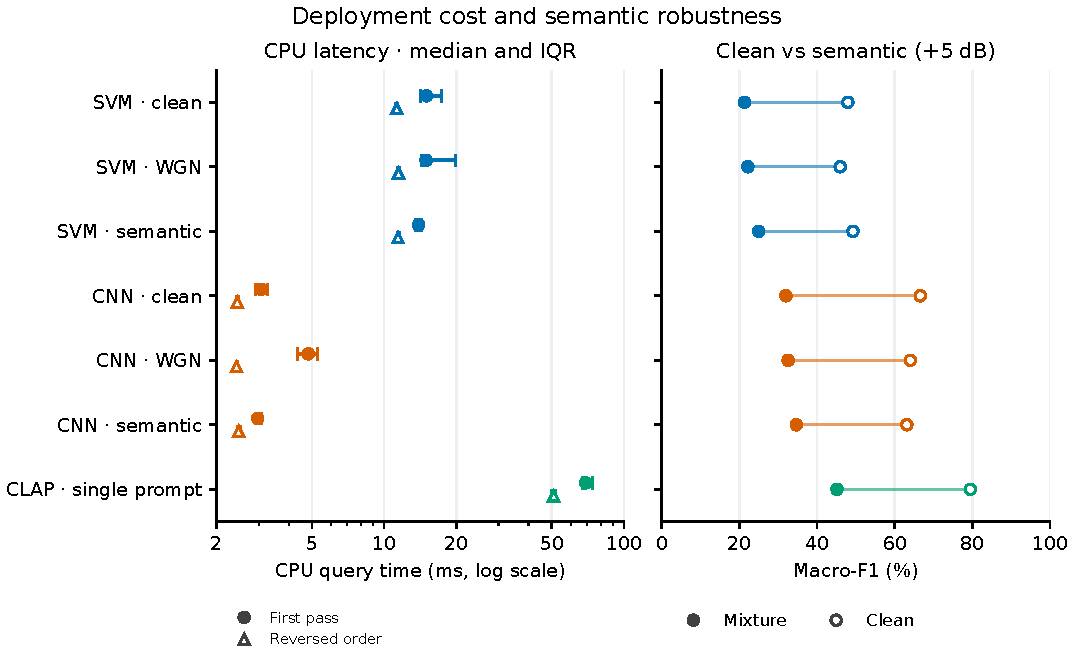
\includegraphics{../results/extensions_20261109/cost_figures/18_balanced_deployment_cost.pdf}
\caption{Balanced CPU latency alongside clean and +5-dB different-category macro-F1 under own-activity power. Both timing passes are retained; whiskers show each pass's interquartile range of 750 queries, not confidence intervals. CNN performance here uses seed 5305; the intervention analysis retains all three seeds.}
\end{figure}
